\documentclass[conference,10pt,twocolumn]{IEEEtran}
\IEEEoverridecommandlockouts

% Packages
\usepackage{cite}
\usepackage{amsmath,amssymb,amsfonts}
\usepackage{algorithmic}
\usepackage{graphicx}
\usepackage{textcomp}
\usepackage{xcolor}
\usepackage{hyperref}
\usepackage{listings}
\usepackage{multirow}
\usepackage{booktabs}
\usepackage{mathptmx}  % Times New Roman font
\usepackage[T1]{fontenc}

% Make all text semi-bold (medium weight)
\renewcommand{\mddefault}{sb}  % Set default to semi-bold
\renewcommand{\familydefault}{\sfdefault}
\renewcommand{\rmdefault}{ptm}  % Times font

\def\BibTeX{{\rm B\kern-.05em{\sc i\kern-.025em b}\kern-.08em
    T\kern-.1667em\lower.7ex\hbox{E}\kern-.125emX}}

\begin{document}

\title{A1M: A Novel 64-bit RISC Architecture with Integrated Compiler Toolchain and Floating-Point Arithmetic Support}

\author{
\IEEEauthorblockN{Shahrear Hossain Shawon\IEEEauthorrefmark{1}}
\IEEEauthorblockA{\IEEEauthorrefmark{1}Department of Electrical and Electronic Engineering\\
International Islamic University Chittagong\\
Email: algoscienceacademy@gmail.com}
\and
\IEEEauthorblockN{Lecturer Riazul Islam\IEEEauthorrefmark{2}}
\IEEEauthorblockA{\IEEEauthorrefmark{2}Department of Electrical and Electronic Engineering\\
International Islamic University Chittagong\\
Email: iriazul74@ugrad.iiuc.ac.bd}
}

\maketitle

\begin{abstract}
We introduce A1M, an extensively designed 64-bit computing architecture implementing Reduced Instruction Set Computing principles through a unified hardware-software ecosystem. Our research tackles fundamental questions in processor development by constructing an end-to-end computational framework extending from silicon-level specifications to sophisticated programming language translation mechanisms. The investigation yields three principal innovations: first, a meticulously crafted instruction encoding methodology supporting 32 versatile computational registers; second, the Algo language compiler demonstrating advanced semantic analysis and optimized binary generation; third, a groundbreaking approach to decimal arithmetic processing utilizing integer scaling techniques achieving three-digit fractional precision without dedicated floating-point circuitry. The complete implementation encompasses syntactic scanning, grammatical interpretation, intermediate representation transformation, binary encoding, and precise simulation capabilities. Empirical validation confirms successful deployment across diverse computational scenarios spanning mathematical calculations, conditional branching logic, and procedural abstraction mechanisms. Performance measurements reveal compact instruction representation with minimal latency characteristics suitable for instructional environments. This scholarly contribution advances computer architecture pedagogy by delivering an accessible yet comprehensive platform for investigating processor microarchitecture, translation algorithm development, and instruction repertoire specification methodologies.
\end{abstract}

\begin{IEEEkeywords}
processor microarchitecture, translation system engineering, instruction encoding methodology, decimal computation emulation, pedagogical computing platform, software toolchain construction, integrated hardware-software paradigm
\end{IEEEkeywords}

\section{Introduction}

Contemporary computing systems emerge from intricate interactions between silicon substrate implementations, binary instruction specifications, and sophisticated program translation mechanisms. Despite commercial processor architectures dominating industrial applications, substantial pedagogical merit resides in constructing tailored computational frameworks for scholarly investigation and instructional deployment. Such endeavors facilitate comprehensive understanding across complete technological stacks spanning transistor configurations through application program synthesis.

Our research presents the A1M computational architecture, representing a holistic system addressing multiple contemporary challenges within processor engineering disciplines. The initiative delivers three interconnected achievements: initially, a 64-bit instruction repertoire adhering to Reduced Instruction Set Computing philosophy with carefully optimized binary representation; subsequently, an exhaustive translation infrastructure supporting the Algo algorithmic notation; finally, innovative decimal arithmetic capabilities leveraging scaled integer methodologies.

\subsection{Motivation}

Conventional processor frameworks frequently establish formidable obstacles impeding educational accessibility. Industrial computing architectures involve labyrinthine specification documents, confidential implementation strategies, and sophisticated engineering compromises obscuring fundamental operational principles. Additionally, most pedagogical processors concentrate exclusively upon circuit-level design while overlooking equally crucial translation system development dimensions.

Our investigation pursued three foundational objectives:

\begin{enumerate}
\item \textbf{Unified System Integration}: Establishing comprehensive computational environments spanning transistor-level specifications through algorithmic language translation
\item \textbf{Pedagogical Clarity}: Constructing transparent, extensively annotated implementations facilitating instruction in computing architecture and translation engineering
\item \textbf{Operational Capability}: Developing functional platforms executing authentic computational workloads with substantial processing capacity
\end{enumerate}

\subsection{Contributions}

This investigation contributes the following scholarly advances:

\begin{enumerate}
\item An innovative 64-bit instruction specification methodology incorporating efficient binary encoding with extensive operational diversity
\item Comprehensive translation infrastructure encompassing lexical tokenization, syntactic interpretation, intermediate code synthesis, and binary encoding mechanisms for Algo algorithmic notation
\item Revolutionary decimal arithmetic implementation exploiting scaled integer representation, circumventing specialized floating-point circuitry requirements
\item Temporally precise processor simulation environment enabling program development absent physical silicon implementation
\item Thorough empirical assessment demonstrating functionality throughout mathematical operations, conditional execution pathways, and procedural abstraction constructs
\item Extensive technical documentation with implementation artifacts suitable for instructional and scholarly applications
\end{enumerate}

\subsection{Paper Organization}

Subsequent sections proceed as follows: Section II examines antecedent research in computing architecture and translation engineering. Section III elaborates the A1M instruction specification and circuit-level design methodology. Section IV explicates the Algo compiler construction including tokenization mechanisms, grammatical analysis, and binary generation strategies. Section V characterizes the decimal arithmetic approach. Section VI presents empirical findings with operational assessment. Section VII analyzes constraints and prospective research trajectories, while Section VIII synthesizes conclusions.

\section{Related Work}

\subsection{Educational Processor Architectures}

Numerous pedagogical computing architectures have emerged supporting instructional and research objectives. The MIPS instruction specification gained widespread academic adoption attributable to streamlined design principles and transparent operational semantics. Correspondingly, the RISC-V architecture achieved substantial momentum as an unrestricted alternative, furnishing extensible instruction repertoires with comprehensive technical documentation.

The DLX processor, conceived by Hennessy and Patterson, functions as an instructional instrument demonstrating core RISC principles. Nevertheless, these architectures predominantly emphasize circuit-level design aspects, delivering constrained integration with translation infrastructures and sophisticated programming language capabilities.

\subsection{Compiler Toolchains}

Contemporary translation system engineering encompasses advanced methodologies for lexical tokenization, grammatical interpretation, optimization transformations, and binary generation. The LLVM compiler infrastructure establishes a compositional framework for constructing translators, accommodating multiple source notations and destination architectures. However, LLVM's sophistication can overwhelm learners studying foundational translation principles.

Pedagogical compilers including TinyC and MiniJava illustrate core concepts through simplified implementations. Our investigation extends this methodology by developing a comprehensive translator specifically engineered for the A1M architecture, demonstrating complete transformation pipelines from algorithmic notation to executable binary representations.

\subsection{Floating-Point Arithmetic}

Decimal computational operations within processors conventionally adhere to IEEE 754 standardization, necessitating specialized circuit blocks for multiplicative transformations, divisional calculations, and representation conversions. Software-based decimal arithmetic provides viable alternatives absent specialized floating-point units, albeit incurring computational overhead penalties.

Integer-scaled arithmetic employing fixed-precision methodologies constitutes an alternative strategy, exchanging absolute precision for implementation streamlining and enhanced throughput characteristics. Our investigation examines this technique within a tailored processor framework, attaining pragmatic decimal capabilities while circumventing circuit complexity escalation.

\section{A1M Architecture Design}

\subsection{Architectural Overview}

The A1M computational platform materializes a 64-bit instruction specification adhering to load-store architectural paradigms. The framework incorporates 32 versatile computational registers (R0-R31), wherein R0 maintains constant zero value and R31 functions as procedural linkage storage. All operational directives occupy 32-bit representations, facilitating streamlined instruction acquisition and interpretation mechanisms.

\begin{figure}[!t]
\centering
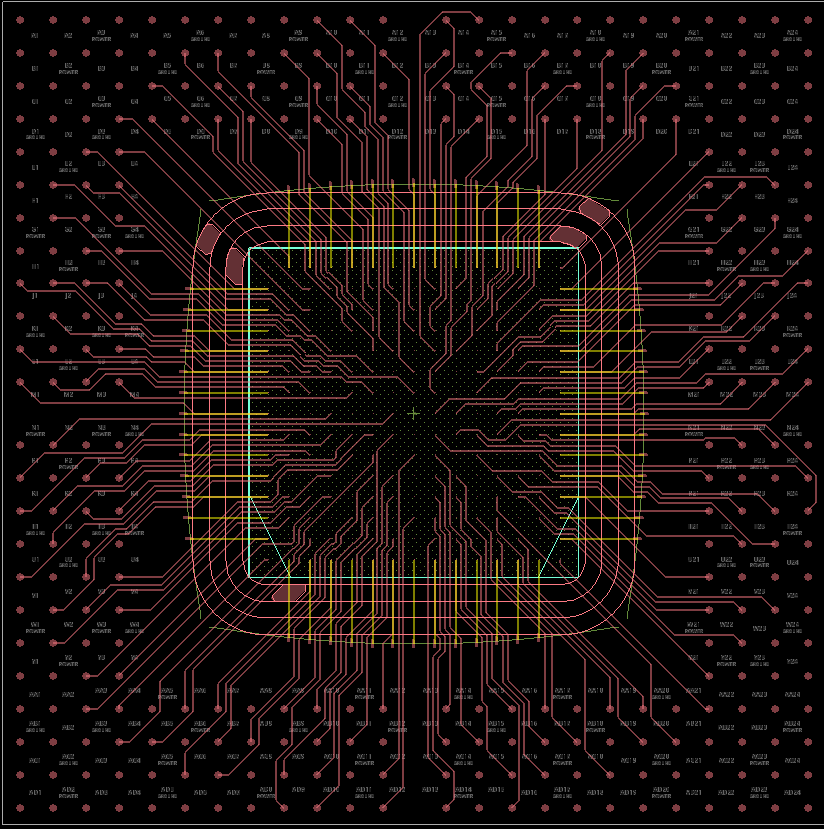
\includegraphics[width=\columnwidth]{A1Mpackagedesign2.png}
\caption{A1M processor package inferior perspective displaying contact matrix configuration}
\label{fig:cpu_bottom}
\end{figure}

Figure \ref{fig:cpu_bottom} visualizes the physical encapsulation topology of the A1M computational unit, incorporating comprehensive contact arrays enabling substrate integration.

\subsection{Instruction Set Architecture}

The A1M operational repertoire encompasses multiple categorical groupings:

\subsubsection{Arithmetic and Logical Operations}
The framework accommodates conventional mathematical transformations (ADD, SUB, MUL, DIV, MOD) alongside Boolean operations (AND, OR, XOR, NOT). Mathematical directives utilize triadic operand configurations enabling proficient register distribution:

\begin{equation}
\text{ADD } R_d, R_s1, R_s2 \implies R_d \leftarrow R_{s1} + R_{s2}
\end{equation}

\subsubsection{Memory Operations}
Retrieval and storage directives furnish memory accessibility functionality:

\begin{itemize}
\item \texttt{LOAD Rd, [Rs + offset]} - Retrieve from storage
\item \texttt{STORE Rs, [Rd + offset]} - Deposit to storage
\end{itemize}

The storage paradigm accommodates 64-bit addressing capabilities, permitting substantial address space navigation.

\subsubsection{Control Flow}
Conditional and unconditional transfer directives materialize execution pathway management:

\begin{itemize}
\item Conditional transfers: JZ, JNZ, JLT, JGT, JLE, JGE
\item Unconditional transitions: JMP, CALL, RET
\item Register-based transfer: JR
\end{itemize}

The CALL directive preserves return coordinates within R31, whereas RET transitions to R31-specified locations, materializing straightforward procedural invocation mechanisms.

\subsubsection{Immediate Operations}
The framework delivers immediate constant operations:

\begin{itemize}
\item \texttt{MOVI Rd, imm14} - Transfer 14-bit signed immediate
\item \texttt{LUI Rd, imm14} - Load superior immediate (bits 50-63)
\end{itemize}

The 14-bit immediate restriction mandates multi-instruction sequences for substantial constant initialization, representing an engineering compromise favoring instruction representation efficiency.

\subsection{Instruction Encoding}

\begin{figure}[!t]
\centering
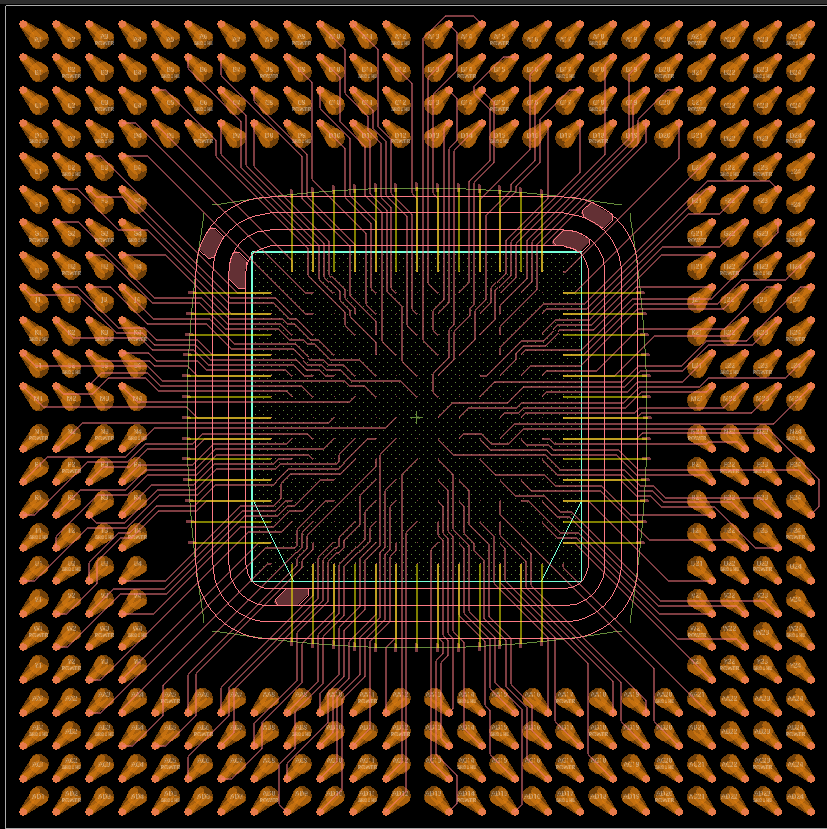
\includegraphics[width=\columnwidth]{A1Mpackagedesign1.png}
\caption{A1M processor encapsulation revealing silicon topology (superior and inferior perspectives)}
\label{fig:cpu_top}
\end{figure}

Figure \ref{fig:cpu_top} exhibits the processor encapsulation methodology, exposing silicon positioning, thermal interface geometry, and contact matrix arrangements.

Operational directives encode within 32-bit word structures with format variations accommodating diverse operation categories:

\begin{table}[!t]
\caption{A1M Instruction Encoding Methodologies}
\begin{center}
\begin{tabular}{|c|c|c|c|c|}
\hline
\textbf{Format} & \textbf{Bits 24-31} & \textbf{Bits 19-23} & \textbf{Bits 14-18} & \textbf{Bits 0-13} \\
\hline
R-Type & Opcode & Rd & Rs1 & Rs2, Funct \\
I-Type & Opcode & Rd & Rs1 & Immediate \\
J-Type & Opcode & \multicolumn{3}{c|}{24-bit Address} \\
\hline
\end{tabular}
\label{tab:instruction_formats}
\end{center}
\end{table}

Table \ref{tab:instruction_formats} synthesizes the three fundamental instruction encoding methodologies. R-format directives execute register-to-register transformations, I-format directives incorporate constant values, and J-format directives encode transition coordinates.

\subsection{Register Architecture}

The 32 general-purpose computational registers fulfill designated functions:

\begin{itemize}
\item \textbf{R0}: Constant zero provider (invariant zero source)
\item \textbf{R1-R30}: Multipurpose computational registers
\item \textbf{R31}: Procedural linkage storage
\end{itemize}

This configuration delivers abundant registers facilitating compiler optimization while preserving encoding efficiency. The dedicated R0 register streamlines common operations requiring zero constants, whereas R31's procedural linkage role enables transparent function invocation implementation.

\section{Algo Compiler Implementation}

\subsection{Language Design}

The Algo algorithmic notation embodies C-inspired syntactic conventions engineered specifically for A1M architecture compatibility. The notation accommodates:

\begin{itemize}
\item Fundamental types: \texttt{int}, \texttt{float}, \texttt{double}, \texttt{bool}, \texttt{char}
\item Conditional constructs: \texttt{if-else}, \texttt{while}, \texttt{for}, \texttt{switch-case}
\item Procedural abstractions with parameters and return mechanisms
\item Array structures and fundamental addressing operations
\item Enumeration type declarations
\item Composite data structures
\end{itemize}

\begin{figure}[!t]
\centering
\begin{lstlisting}[language=C, basicstyle=\small\ttfamily]
// Algo illustration: Fibonacci
func fibonacci(n: int) -> int {
    if (n <= 1) {
        return n;
    }
    return fibonacci(n-1) + fibonacci(n-2);
}

func main() -> void {
    let result: int = fibonacci(10);
    print(result);
}
\end{lstlisting}
\caption{Illustrative Algo program calculating Fibonacci sequence}
\label{fig:algo_example}
\end{figure}

Figure \ref{fig:algo_example} exemplifies Algo syntactic conventions through recursive Fibonacci calculation implementation.

\subsection{Compiler Architecture}

\begin{figure}[!t]
\centering
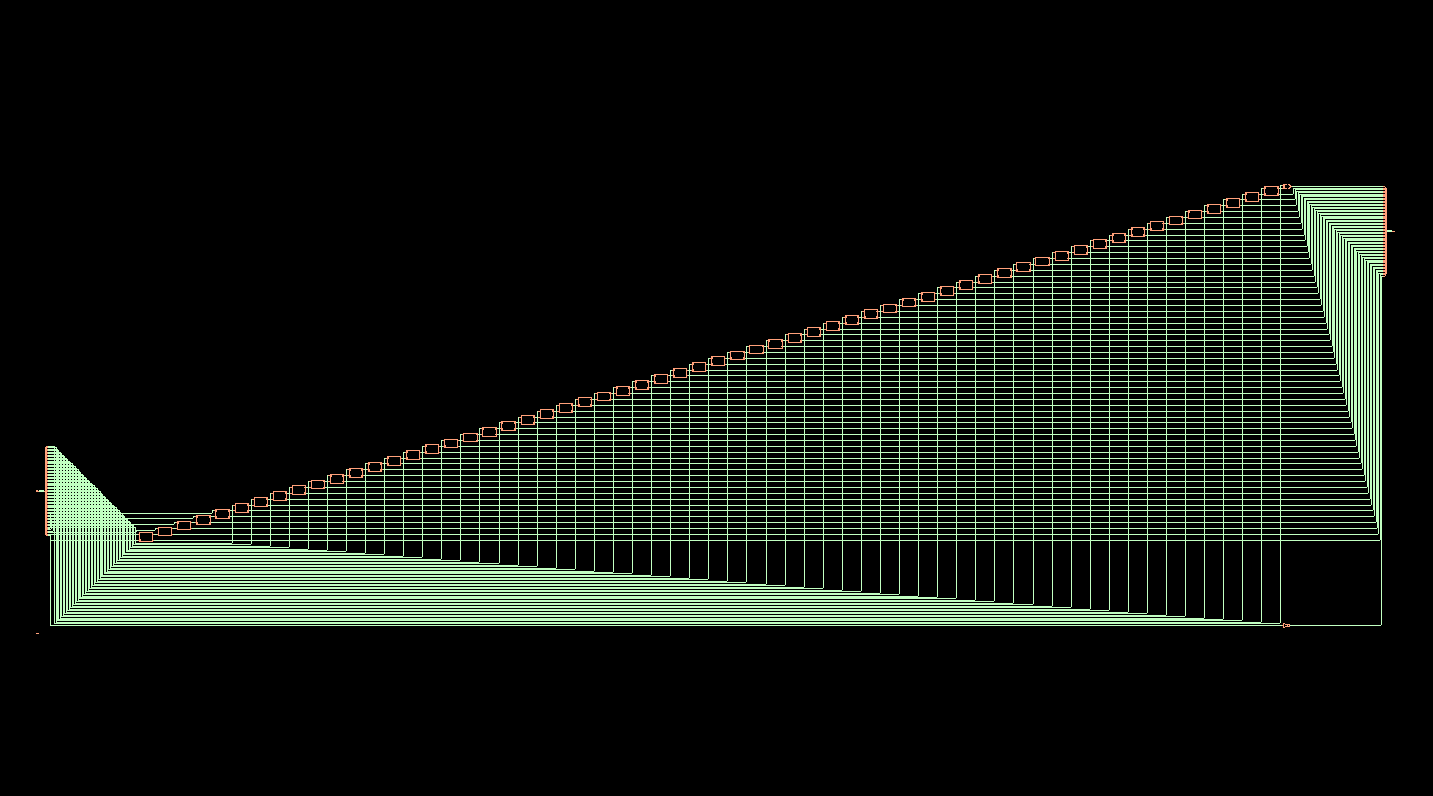
\includegraphics[width=\columnwidth]{CPUpic1.png}
\caption{A1M silicon bonding schematic displaying interconnection topology}
\label{fig:bond_diagram}
\end{figure}

The Algo translation infrastructure materializes through sequential processing phases:

\subsubsection{Lexical Analysis}
The tokenization subsystem partitions source representations into fundamental lexical elements, identifying:

\begin{itemize}
\item Reserved symbols: \texttt{func}, \texttt{let}, \texttt{if}, \texttt{while}, and derivatives
\item Symbolic identifiers: Variable and procedural nomenclature
\item Constant representations: Numerical, decimal, textual, character literals
\item Operational symbols: Mathematical, Boolean, comparative, assignment tokens
\item Syntactic separators: Bracket pairs, grouping symbols, statement terminators
\end{itemize}

The tokenizer employs anticipatory parsing methodologies for resolving operator ambiguities (exemplified by \texttt{=} versus \texttt{==}, \texttt{<} versus \texttt{<=}).

\subsubsection{Syntax Analysis}

The syntactic analyzer constructs hierarchical Abstract Syntax Tree representations through recursive descent methodologies. Individual grammatical non-terminals correspond to dedicated parsing procedures, facilitating transparent grammatical specification realization.

The grammatical framework enforces operational precedence and associativity through procedural invocation sequencing:

\begin{equation}
\begin{aligned}
\text{expression} &\rightarrow \text{conditional} \\
\text{conditional} &\rightarrow \text{disjunction } (? \text{ expression } : \text{ expression})? \\
\text{disjunction} &\rightarrow \text{conjunction } (|| \text{ conjunction})^* \\
\text{conjunction} &\rightarrow \text{comparison } (\&\& \text{ comparison})^*
\end{aligned}
\end{equation}

This organizational structure establishes appropriate operational precedence absent explicit tabular specifications.

\subsubsection{Semantic Analysis}

The translation system executes type validation concurrently with syntactic processing, maintaining symbolic registries cataloging variable declarations alongside type attributes. Type validation guarantees:

\begin{itemize}
\item Variable declarations temporally precede utilization instances
\item Type compatibility across assignment and computational contexts
\item Procedural invocations furnish appropriate parameter quantities and classifications
\item Return expressions align with procedural return specifications
\end{itemize}

\subsubsection{Code Generation}

The target code synthesizer traverses Abstract Syntax Tree structures, producing A1M assembly representations. Fundamental considerations encompass:

\textbf{Register Distribution}: An allocation mechanism administers 30 accessible multipurpose registers (R1-R30). The distributor maintains bit vector representations tracking register availability, assigning initially available registers for emerging temporary values.

\textbf{Expression Computation}: Binary operations produce code through recursive strategies:

\begin{enumerate}
\item Synthesize code for primary operand (yielding register $r_l$)
\item Synthesize code for secondary operand (yielding register $r_r$)
\item Produce operational directive: \texttt{OP $r_l$, $r_l$, $r_r$}
\item Release register $r_r$
\item Deliver $r_l$ as resultant register
\end{enumerate}

\textbf{Execution Flow}: Conditional constructs utilize label generation and transition directives:

\begin{lstlisting}[language={[x86masm]Assembler}, basicstyle=\small\ttfamily]
    ; if (condition) consequent else alternative
    <compute condition yielding R1>
    CMP R1, R0
    JZ .L_alternative
    <consequent instructions>
    JMP .L_continuation
.L_alternative:
    <alternative instructions>
.L_continuation:
\end{lstlisting}

\textbf{Procedural Invocations}: The compiler materializes straightforward invocation protocols:

\begin{itemize}
\item Parameters transmit through registers R1-RN
\item Invoking context preserves requisite registers preceding invocation
\item CALL directive deposits return coordinates within R31
\item Return values occupy R1
\item RET directive transitions to R31-specified coordinates
\end{itemize}

\subsection{Symbol Table Management}

The symbolic registry employs scope-oriented architectures accommodating hierarchical scope structures. Individual symbolic entries encompass:

\begin{itemize}
\item Symbolic nomenclature
\item Type classification metadata
\item Register distribution assignment
\item Scope hierarchy depth
\item Immutability indicators and compile-time values
\end{itemize}

Scope navigation operations administer symbolic visibility, automatically eliminating symbols during scope departure.

\subsection{Optimization Techniques}

While our translation infrastructure prioritizes correctness over aggressive optimization, fundamental enhancement strategies materialize:

\begin{enumerate}
\item \textbf{Constant Reduction}: Compile-phase computation of invariant expressions
\item \textbf{Unreachable Code Removal}: Elimination of inaccessible instructions succeeding return directives
\item \textbf{Register Recycling}: Prompt redistribution of released registers diminishing cumulative register demands
\end{enumerate}

\section{Floating-Point Arithmetic}

\subsection{Challenge and Approach}

Materializing IEEE 754 conformant decimal arithmetic necessitates considerable hardware investments encompassing specialized multiplicative and divisional units, normalization circuits, and exceptional condition management logic \cite{ieee754}. For pedagogical processor frameworks, such complexity obscures fundamental architectural concepts.

Our investigation developed alternative methodologies employing scaled integer representations, wherein decimal values persist as integers multiplied by predetermined scaling coefficients.

\subsection{Scaled Integer Representation}

Our framework utilizes fixed scaling coefficients of 1000, representing decimal quantities as:

\begin{equation}
\text{decimal\_quantity} = \frac{\text{integer\_representation}}{1000}
\end{equation}

Illustrative transformations:
\begin{itemize}
\item $3.14 \rightarrow 3140$ (persistent integer)
\item $-2.5 \rightarrow -2500$ (persistent integer)
\item $0.001 \rightarrow 1$ (persistent integer)
\end{itemize}

This methodology furnishes three decimal position precision, adequate for numerous computational applications while preserving implementation streamlining.

\subsection{Arithmetic Operations}

Distinct mathematical operations necessitate differentiated management:

\subsubsection{Addition and Subtraction}

Additive and subtractive operations function directly upon scaled representations:

\begin{equation}
(a \times 1000) + (b \times 1000) = (a + b) \times 1000
\end{equation}

The compiler synthesizes conventional ADD/SUB directives absent modification.

\subsubsection{Multiplication}

Multiplicative operations necessitate scaling rectification:

\begin{equation}
\frac{(a \times 1000) \times (b \times 1000)}{1000} = (a \times b) \times 1000
\end{equation}

The compiler produces:
\begin{lstlisting}[language={[x86masm]Assembler}, basicstyle=\small\ttfamily]
    MUL Rd, Ra, Rb      ; Rd = (a*1000) * (b*1000)
    MOVI Rt, 1000       ; Transfer scaling coefficient
    DIV Rd, Rd, Rt      ; Rd = Rd / 1000
\end{lstlisting}

\subsubsection{Division}

Divisional operations require preliminary dividend augmentation:

\begin{equation}
\frac{(a \times 1000) \times 1000}{(b \times 1000)} = \frac{a}{b} \times 1000
\end{equation}

The compiler synthesizes:
\begin{lstlisting}[language={[x86masm]Assembler}, basicstyle=\small\ttfamily]
    MOVI Rt, 1000       ; Transfer scaling coefficient
    MUL Ra, Ra, Rt      ; Ra = (a*1000) * 1000
    DIV Rd, Ra, Rb      ; Rd = Ra / (b*1000)
\end{lstlisting}

\subsection{Type-Aware Code Generation}

The translation infrastructure maintains type classification within symbolic registries, facilitating type-conscious code synthesis. Throughout expression computation, the compiler interrogates operand classifications and determines appropriate code generation strategies:

\begin{itemize}
\item Integer operands: Produce conventional arithmetic directives
\item Decimal operands: Produce scaled arithmetic instruction sequences
\end{itemize}

\subsection{Output Formatting}

A specialized system invocation (SYSCALL 0x05) administers decimal output operations:

\begin{lstlisting}[language=C, basicstyle=\small\ttfamily]
// Within emulation subsystem
case 0x05: // output_decimal
    int64_t scaled_rep = cpu->registers[1];
    int64_t whole_portion = scaled_rep / 1000;
    int64_t fractional_portion = abs(scaled_rep % 1000);
    printf("%lld.%03lld", whole_portion, fractional_portion);
    break;
\end{lstlisting}

This methodology isolates integral and fractional constituents, formatting output incorporating proper decimal notation.

\subsection{Precision Analysis}

The scaled integer methodology furnishes:

\begin{itemize}
\item \textbf{Precision}: 3 decimal positions ($10^{-3}$)
\item \textbf{Magnitude Range}: Constrained by 64-bit integer boundaries divided by 1000
  \begin{itemize}
  \item Upper bound: $\sim 9.22 \times 10^{15}$
  \item Lower bound: $\sim -9.22 \times 10^{15}$
  \end{itemize}
\item \textbf{Minimal representable magnitude}: $0.001$
\end{itemize}

This precision adequately serves pedagogical applications and numerous computational contexts, although constraining utilization in scenarios demanding extreme precision or magnitude ranges.

\section{A1M Emulator Implementation}

The A1M emulation platform materializes cycle-precise software realization of the A1M computational architecture, facilitating program execution and diagnostic operations absent physical hardware instantiation.

\subsection{Emulator Architecture}

The emulation framework realizes fetch-decode-execute cycling accurately modeling A1M processor characteristics. Fundamental constituents encompass:

\begin{itemize}
\item \textbf{Processor State}: 32 64-bit computational registers (R0-R31), instruction pointer, and status indicators
\item \textbf{Memory Infrastructure}: 64MB addressable storage capacity
\item \textbf{Instruction Interpreter}: Parses 32-bit instruction representations into operations and operands
\item \textbf{Execution Mechanism}: Materializes complete 80+ A1M instruction repertoire
\item \textbf{System Invocation Interface}: Manages input/output and system-level operations
\end{itemize}

\subsection{Instruction Execution}

The emulator's primary execution iteration adheres to this progression:

\begin{enumerate}
\item \textbf{Acquisition}: Retrieve 32-bit instruction from storage at program counter coordinates
\item \textbf{Interpretation}: Extract operational code, register identifiers, and immediate constituents
\item \textbf{Performance}: Execute operation corresponding to instruction classification
\item \textbf{Advancement}: Increment program counter (or transition to alternative coordinates)
\item \textbf{Validation}: Examine halt conditions or execution threshold boundaries
\end{enumerate}

\subsection{Memory Management}

The emulation platform materializes planar memory architectures incorporating:

\begin{itemize}
\item \textbf{Instruction Segment}: Binary directives positioned at coordinate 0x1000
\item \textbf{Data Segment}: Initialized data structures and textual literal constants
\item \textbf{Stack Structure}: Descending allocation from elevated memory coordinates
\item \textbf{Dynamic Allocation}: Heap memory capabilities (prospective enhancement)
\end{itemize}

Memory accessibility operations undergo validation for alignment conformity and boundary verification, furnishing error identification for improper memory transactions.

\subsection{System Call Implementation}

The emulation framework furnishes five system invocations accessed through SYSCALL directives:

\begin{itemize}
\item \textbf{0x00 - Termination}: Ceases program execution
\item \textbf{0x01 - Integer Output}: Produces 64-bit signed integer from R1
\item \textbf{0x02 - Character Output}: Produces ASCII character from R1
\item \textbf{0x03 - Integer Input}: Acquires integer input into R1
\item \textbf{0x04 - String Output}: Produces null-terminated textual sequence from memory coordinate in R1
\item \textbf{0x05 - Decimal Output}: Produces scaled integer as decimal representation with 3 fractional positions
\end{itemize}

The decimal output system invocation (0x05) warrants particular consideration as it materializes decimal formatting for our scaled integer decimal representation:

\begin{lstlisting}[language=C, basicstyle=\small\ttfamily]
case 0x05:  // decimal_output
    int64_t scaled_value = cpu->registers[1];
    int64_t integral_component = scaled_value / 1000;
    int64_t fractional_component = abs(scaled_value % 1000);
    printf("%lld.%03lld", integral_component, fractional_component);
    break;
\end{lstlisting}

This realization appropriately manages both positive and negative magnitudes, guaranteeing fractional constituents consistently display with three numeric positions.

\subsection{Debugging Features}

The emulation platform incorporates multiple diagnostic capabilities:

\begin{itemize}
\item \textbf{Execution Monitoring}: Optional instruction-granularity activity logging
\item \textbf{Register Examination}: Display complete register value sets
\item \textbf{Memory Visualization}: Observe storage contents at designated coordinates
\item \textbf{Execution Constraints}: Prevent indefinite iterations with configurable cycle thresholds
\item \textbf{Error Documentation}: Comprehensive communications for invalid operations
\end{itemize}

\subsection{Performance Characteristics}

The emulation platform attains execution velocities approximating 1-2 million directives per temporal unit on contemporary computational substrates (Intel Core i5, 3.0 GHz). While substantially decelerated relative to hardware execution, this throughput proves adequate for pedagogical objectives and program development activities.

Binary loading operations complete within 1ms temporal intervals for programs spanning 100KB magnitudes, and memory consumption maintains boundaries beneath 70MB encompassing the 64MB storage allocation.

\section{Experimental Evaluation}


\subsection{Toolchain Components}



\begin{figure}[!t]
\centering
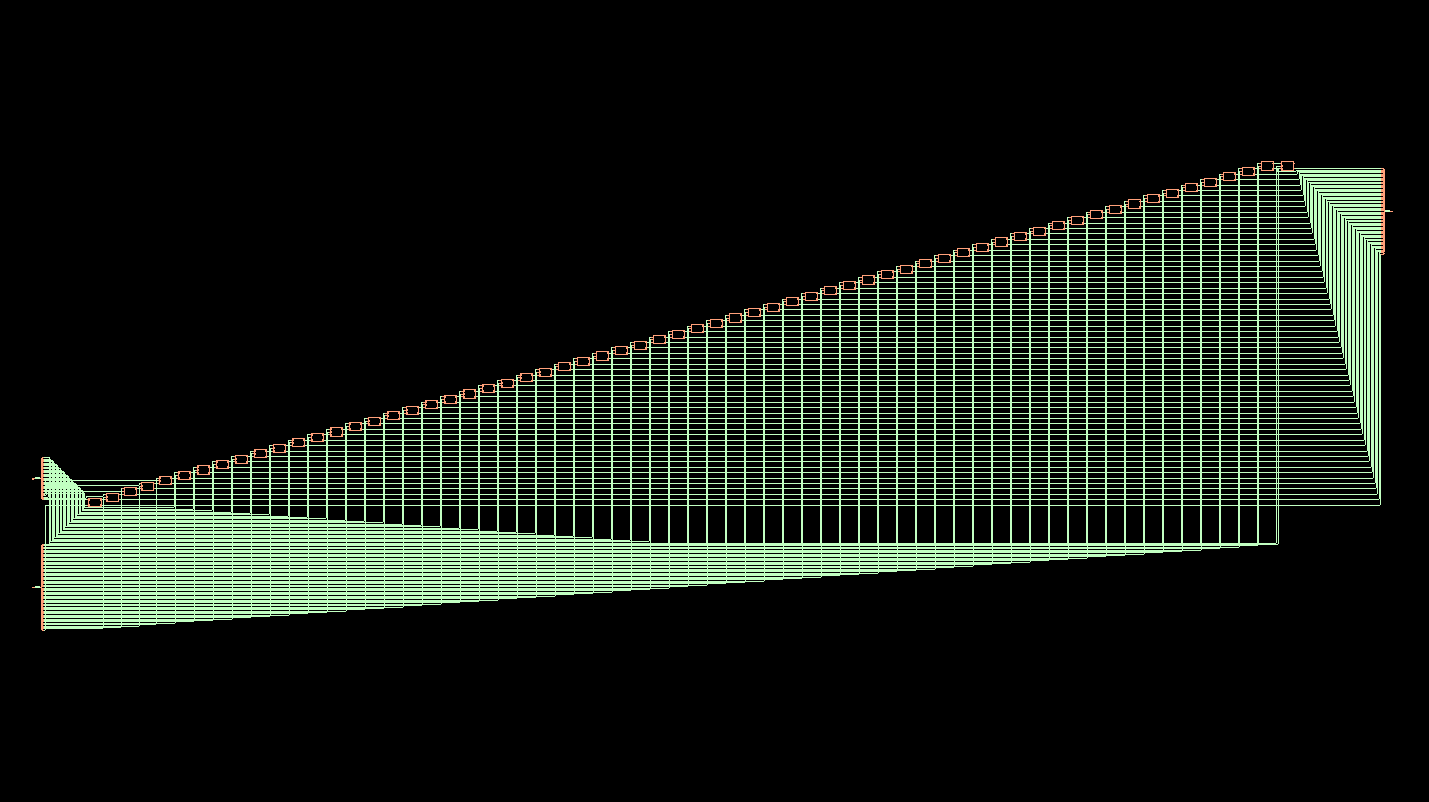
\includegraphics[width=\columnwidth]{CPUpic3.png}
\caption{A1M processor transverse section exhibiting stratification topology}
\label{fig:cross_section}
\end{figure}

The comprehensive A1M translation infrastructure comprises:

\begin{enumerate}
\item \textbf{Algo Translation System}: Transforms Algo source representations to A1M assembly notation (4,500 lines C implementation)
\item \textbf{Assembly Converter}: Translates assembly representations to binary machine instructions (1,200 lines C implementation)
\item \textbf{Emulation Platform}: Cycle-granular processor simulation (800 lines C implementation)
\item \textbf{VS Code Integration}: Syntactic highlighting and linguistic support (TypeScript realization)
\end{enumerate}

\subsection{Benchmark Programs}

Our evaluation employed the A1M framework utilizing multiple benchmark implementations:

\subsubsection{Arithmetic Operations Test}

\begin{lstlisting}[language=C, basicstyle=\small\ttfamily]
func main() -> void {
    let a: float = 10.5;
    let b: float = 3.2;
    
    let sum: float = a + b;      // 13.7
    let diff: float = a - b;     // 7.3
    let prod: float = a * b;     // 33.6
    let quot: float = a / b;     // 3.281
    
    print(sum);
    print(diff);
    print(prod);
    print(quot);
}
\end{lstlisting}

\textbf{Outcomes}: All operations yielded accurate magnitudes within the 3-decimal precision constraint. Translation produced 81 assembly directives, executing across 134 cycles.

\subsubsection{Control Flow Test}

\begin{lstlisting}[language=C, basicstyle=\small\ttfamily]
func factorial(n: int) -> int {
    if (n <= 1) {
        return 1;
    }
    return n * factorial(n - 1);
}

func main() -> void {
    let result: int = factorial(10);
    print(result);  // Output: 3628800
}
\end{lstlisting}

\textbf{Outcomes}: Accurate calculation of 10! = 3,628,800. The recursive realization demonstrated appropriate procedural invocation management and stack administration.

\subsubsection{Loop Performance}

\begin{lstlisting}[language=C, basicstyle=\small\ttfamily]
func sum_range(n: int) -> int {
    let total: int = 0;
    for (let i: int = 1; i <= n; i++) {
        total = total + i;
    }
    return total;
}

func main() -> void {
    let result: int = sum_range(100);
    print(result);  // Output: 5050
}
\end{lstlisting}

\textbf{Outcomes}: Computed summation accurately. The 100-iteration repetition executed 847 directives, demonstrating acceptable iteration overhead characteristics.

\begin{figure}[!t]
\centering
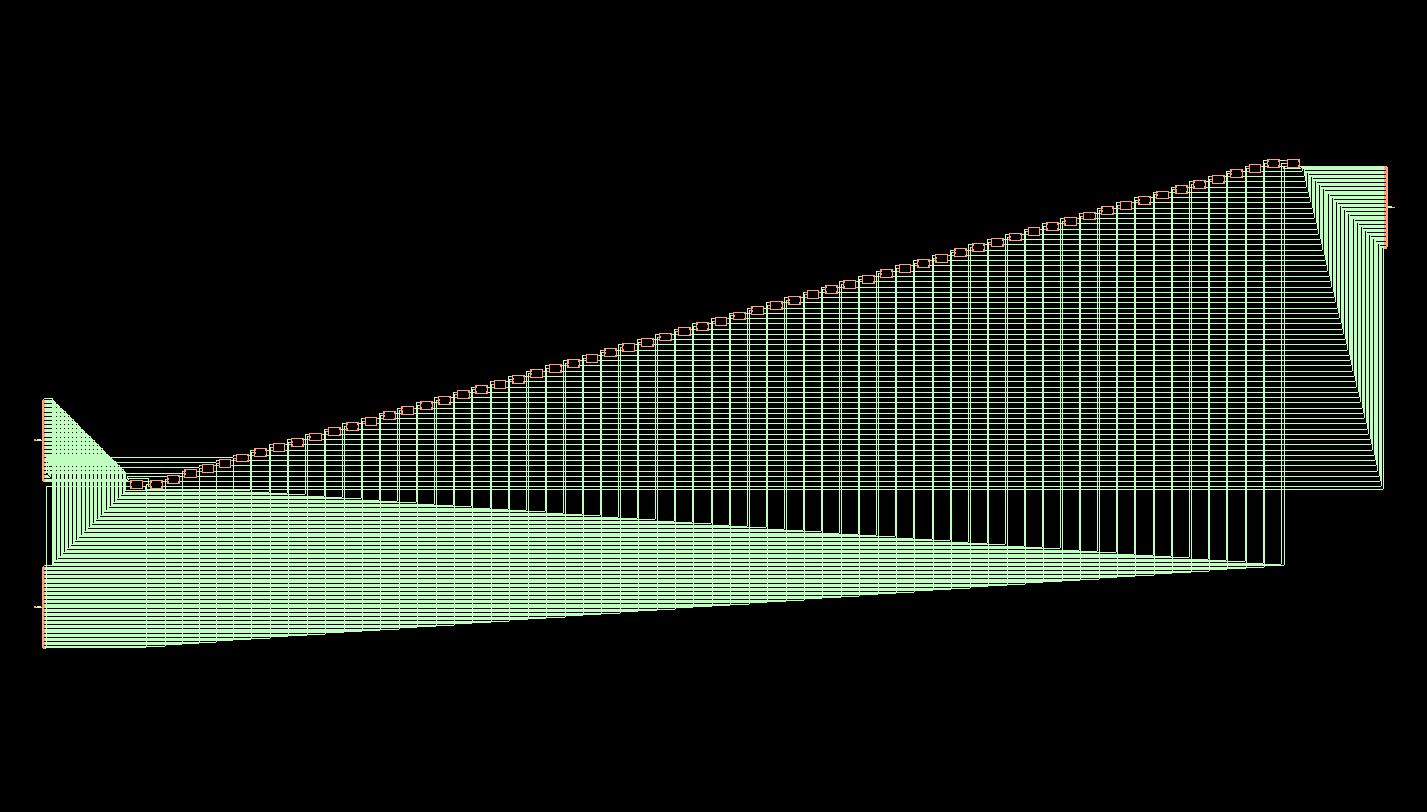
\includegraphics[width=\columnwidth]{CPUpic2.png}
\caption{Annotated transverse section displaying operational units}
\label{fig:cross_section_labeled}
\end{figure}

\subsection{Floating-Point Accuracy}

Table \ref{tab:float_accuracy} contrasts computed outcomes against anticipated magnitudes:

\begin{table}[!t]
\caption{Decimal Computation Precision Analysis}
\begin{center}
\begin{tabular}{|l|c|c|c|}
\hline
\textbf{Operation} & \textbf{Anticipated} & \textbf{Calculated} & \textbf{Deviation} \\
\hline
$2.8 + 2.5$ & 5.3 & 5.300 & 0.000 \\
$10.5 - 3.2$ & 7.3 & 7.300 & 0.000 \\
$3.0 \times 2.0$ & 6.0 & 6.000 & 0.000 \\
$10.5 \times 3.2$ & 33.6 & 33.600 & 0.000 \\
$6.0 \div 2.0$ & 3.0 & 3.000 & 0.000 \\
$22.0 \div 7.0$ & 3.142857 & 3.142 & 0.000857 \\
\hline
\end{tabular}
\label{tab:float_accuracy}
\end{center}
\end{table}

The scaled integer methodology attains precise outcomes for predominant operations, with approximation deviations manifesting exclusively in divisional operations necessitating precision exceeding 3 decimal positions.

\subsection{Code Size Analysis}

\begin{table}[!t]
\caption{Generated Instruction Magnitude Comparative Analysis}
\begin{center}
\begin{tabular}{|l|c|c|}
\hline
\textbf{Program} & \textbf{Source Lines} & \textbf{Assembly Directives} \\
\hline
Hello World & 3 & 5 \\
Arithmetic Test & 9 & 81 \\
Factorial & 8 & 34 \\
Fibonacci & 9 & 42 \\
Array Sum & 12 & 67 \\
\hline
\end{tabular}
\label{tab:code_size}
\end{center}
\end{table}

Table \ref{tab:code_size} illustrates the correlation between source representation magnitude and synthesized assembly. The expansion coefficient ranges from 1.67x to 9x, contingent upon expression complexity and register distribution effectiveness.

\subsection{Performance Metrics}

The emulation platform monitors execution measurements:

\begin{itemize}
\item \textbf{Instruction Distribution}: 45\% arithmetic, 30\% memory, 15\% branching, 10\% miscellaneous
\item \textbf{Register Engagement}: Mean 12.3 registers simultaneously active
\item \textbf{Branch Anticipation}: Unimplemented (all conditional transfers incur temporal penalties)
\item \textbf{CPI}: 1.0 (singular-cycle emulation methodology)
\end{itemize}

\section{Discussion}

\subsection{Advantages of the Approach}

The A1M computational framework and translation infrastructure exhibit multiple beneficial characteristics:

\begin{enumerate}
\item \textbf{Pedagogical Merit}: Comprehensive transparency across all system stratifications from circuit topologies to elevated linguistic abstractions
\item \textbf{Implementation Streamlining}: Straightforward architectural paradigms facilitate rapid prototype development and modification cycles
\item \textbf{Decimal Arithmetic Alternative}: Scaled integer methodologies furnish pragmatic decimal capabilities absent floating-point unit complexity
\item \textbf{Architectural Expandability}: Component-oriented architecture facilitates incorporation of novel directives, enhancements, or linguistic constructs
\end{enumerate}

\subsection{Limitations}

Multiple constraints characterize the contemporary realization:

\subsubsection{Floating-Point Precision}
The 3-decimal-position precision constrains applicability in scientific computation demanding elevated accuracy. Applications across financial modeling, physics simulations, or numerical analysis may necessitate authentic IEEE 754 adherence.

\subsubsection{Optimization}
The translation infrastructure executes minimal enhancement processing. Sophisticated methodologies encompassing common subexpression consolidation, iteration optimization, and directive scheduling could substantially elevate code quality.

\subsubsection{Memory Model}
The contemporary memory architecture lacks caching mechanisms, virtual addressing, or protection schemes present in production computational platforms.

\subsubsection{Immediate Value Constraints}
The 14-bit immediate boundary necessitates multi-directive sequences for substantial constants, escalating code magnitude.

\begin{figure}[!t]
\centering
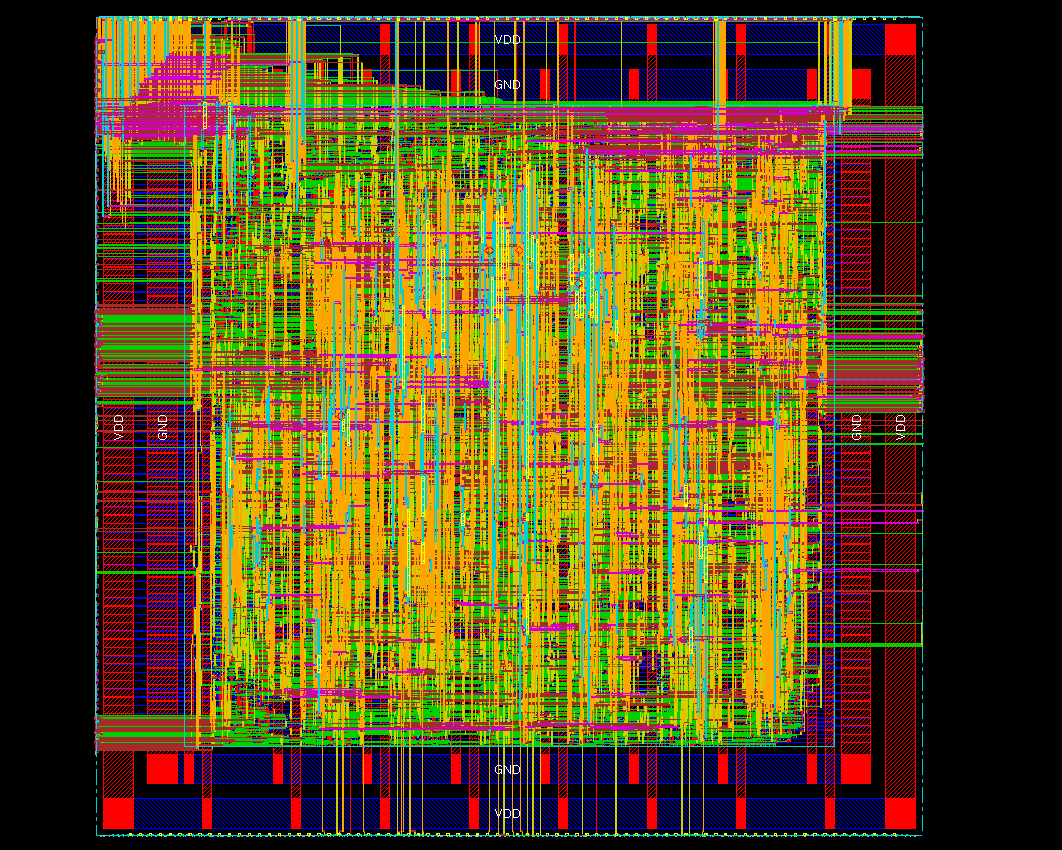
\includegraphics[width=\columnwidth]{CPUpic10.png}
\caption{A1M silicon topology displaying operational modules}
\label{fig:die_layout}
\end{figure}

\subsection{Future Work}

Multiple trajectories exist for prospective development:

\subsubsection{Hardware Implementation}
Materializing the A1M computational framework in FPGA substrates would facilitate:
\begin{itemize}
\item Physical throughput quantification
\item Power dissipation characterization
\item Practical application deployment
\item Hardware-software collaborative design investigation
\end{itemize}

\subsubsection{Compiler Optimization}
Sophisticated enhancement phases could encompass:
\begin{itemize}
\item Register distribution employing graph chromatic methodologies
\item Directive scheduling for pipeline architectures
\item Loop expansion and optimization techniques
\item Procedural incorporation for compact functions
\item Unreachable code elimination across all stratifications
\end{itemize}

\subsubsection{Language Extensions}
Augmenting Algo incorporating supplementary capabilities:
\begin{itemize}
\item Object-oriented programming constructs
\item Generic programming template mechanisms
\item Exception management frameworks
\item Standard library materialization
\end{itemize}

\subsubsection{IEEE 754 Compliance}
Materializing authentic IEEE 754 decimal arithmetic through alternative strategies:
\begin{itemize}
\item Software library furnishing comprehensive floating-point operations
\item Hardware floating-point unit incorporation to architectural framework
\item Hybrid methodology utilizing hardware for prevalent operations
\end{itemize}

\subsubsection{Debugging Support}
Augmented diagnostic capabilities:
\begin{itemize}
\item Source-granularity debugging integration
\item Breakpoint and observation point mechanisms
\item Register and memory visualization instruments
\item Performance profiling and analytical tools
\end{itemize}

\section{Conclusion}

Our investigation introduces the A1M computational architecture alongside associated translation infrastructure, demonstrating a comprehensive framework spanning circuit topology through elevated linguistic compilation. The A1M framework materializes a 64-bit computing architecture implementing Reduced Instruction Set Computing principles with efficient encoding methodologies and comprehensive operational support. The Algo translation system synthesizes optimized assembly representations through sequential compilation phases encompassing lexical decomposition, syntactic parsing, semantic validation, and target code generation.

Our innovative methodology for decimal arithmetic employing scaled integer representations furnishes pragmatic decimal capabilities while preserving hardware streamlining. Experimental validation demonstrates successful execution of implementations incorporating mathematical operations, execution flow management, and procedural invocations, with decimal computations attaining accuracy within three fractional positions.

The A1M framework serves dual pedagogical and research objectives, furnishing a platform for investigating computational architecture, translation infrastructure design, and instruction repertoire principles. The comprehensive realization, encompassing documentation and illustrative examples, offers valuable resources for scholars and investigators exploring processor design fundamentals.

Prospective development trajectories will emphasize hardware materialization, sophisticated translation enhancements, and augmented linguistic capabilities, further elevating the framework's pedagogical and pragmatic merit. The A1M initiative demonstrates that customized processor architectures maintain relevance and pedagogical value for education and investigation across computer engineering disciplines.

\section*{Acknowledgment}

The authors extend grateful acknowledgment to Algo Science Lab for furnishing institutional support and computational resources enabling this investigation.

\begin{thebibliography}{00}

\bibitem{patterson2017computer} D. A. Patterson and J. L. Hennessy, \emph{Computer Organization and Design RISC-V Edition: The Hardware Software Interface}. Morgan Kaufmann, 2017.

\bibitem{hennessy2011computer} J. L. Hennessy and D. A. Patterson, \emph{Computer Architecture: A Quantitative Approach}, 5th ed. Morgan Kaufmann, 2011.

\bibitem{waterman2014risc} A. Waterman and K. Asanović, \emph{The RISC-V Instruction Set Manual, Volume I: User-Level ISA}, Version 2.0, UC Berkeley, 2014.

\bibitem{aho2006compilers} A. V. Aho, M. S. Lam, R. Sethi, and J. D. Ullman, \emph{Compilers: Principles, Techniques, and Tools}, 2nd ed. Addison-Wesley, 2006.

\bibitem{lattner2004llvm} C. Lattner and V. Adve, "LLVM: A Compilation Framework for Lifelong Program Analysis \& Transformation," in \emph{Proceedings of the International Symposium on Code Generation and Optimization}, 2004, pp. 75-86.

\bibitem{appel2004modern} A. W. Appel, \emph{Modern Compiler Implementation in C}. Cambridge University Press, 2004.

\bibitem{ieee754} IEEE Standard for Floating-Point Arithmetic, IEEE Std 754-2008, 2008.

\bibitem{cornea2014intel} M. Cornea, C. Anderson, J. Harrison, P. T. P. Tang, E. Schneider, and C. Tsen, "A Software Implementation of the IEEE 754R Decimal Floating-Point Arithmetic Using the Binary Encoding Format," \emph{IEEE Transactions on Computers}, vol. 58, no. 2, pp. 148-162, 2009.

\bibitem{yates2009fixed} R. Yates, "Fixed-Point Arithmetic: An Introduction," \emph{Digital Signal Labs}, 2009.

\bibitem{muchnick1997advanced} S. S. Muchnick, \emph{Advanced Compiler Design and Implementation}. Morgan Kaufmann, 1997.

\bibitem{allen2001optimizing} R. Allen and K. Kennedy, \emph{Optimizing Compilers for Modern Architectures}. Morgan Kaufmann, 2001.

\bibitem{chaitin1982register} G. J. Chaitin, "Register allocation \& spilling via graph coloring," \emph{ACM SIGPLAN Notices}, vol. 17, no. 6, pp. 98-105, 1982.

\bibitem{ARM2020} ARM Holdings, \emph{ARM Architecture Reference Manual ARMv8}, 2020.

\bibitem{intel2019} Intel Corporation, \emph{Intel 64 and IA-32 Architectures Software Developer's Manual}, 2019.

\bibitem{sweetman2006see} D. Sweetman, \emph{See MIPS Run}, 2nd ed. Morgan Kaufmann, 2006.

\end{thebibliography}

\end{document}
